% ============================================================
%  CHAPTER: Understanding Your Risk Profile
%  Part of: Beginner's Guide to Selecting Mutual Funds
%  Sources: Rachel Ranade, Yadnya Investment Academy,
%           IMD Learn, Risk Analysis Test Framework
% ============================================================

\documentclass[12pt,a4paper]{article}

% ── Packages ─────────────────────────────────────────────────
\usepackage[utf8]{inputenc}
\usepackage[T1]{fontenc}
\newcommand{\rupee}{Rs.\@}
\usepackage[a4paper, top=25mm, bottom=25mm,
            left=22mm, right=22mm]{geometry}
\usepackage{amsmath,amssymb}
\usepackage[table,dvipsnames]{xcolor}
\usepackage{tcolorbox}
\tcbuselibrary{skins,breakable,theorems}
\usepackage{enumitem}
\usepackage{booktabs}
\usepackage{tabularx}
\usepackage{array}
\newcolumntype{L}[1]{>{\raggedright\arraybackslash}p{#1}}
\newcolumntype{B}[1]{>{\bfseries\raggedright\arraybackslash}p{#1}}
\newcolumntype{Y}{>{\raggedright\arraybackslash}X}
\usepackage{multicol}
\usepackage{pifont}
\newcommand{\faCalendar}{\ding{111}}
\newcommand{\faPiggyBank}{\ding{108}}
\newcommand{\faBriefcase}{\ding{115}}
\newcommand{\faChartLine}{\ding{116}}
\newcommand{\faBookmark}{\ding{228}}
\newcommand{\faLightbulb}{\ding{42}}
\newcommand{\faExclamationTriangle}{\ding{54}}
\newcommand{\faKey}{\ding{166}}
\newcommand{\faStickyNote}{\ding{113}}
\newcommand{\faShield}{\ding{110}}
\newcommand{\faShieldx}{\ding{110}}
\newcommand{\faShieldStar}{\faShield}
\newcommand{\faBalanceScale}{\ding{202}}
\newcommand{\faRocket}{\ding{225}}
\usepackage{tikz}
\usetikzlibrary{arrows.meta,shapes,positioning,fit,backgrounds,
                decorations.pathmorphing}
\usepackage{hyperref}
\hypersetup{colorlinks=true, linkcolor=NavyBlue, urlcolor=NavyBlue}
\usepackage{parskip}
%\usepackage{microtype}
\usepackage{mdframed}
\usepackage{needspace}

% ── Colour palette ───────────────────────────────────────────
\definecolor{PrimaryBlue}{HTML}{1A3C6E}
\definecolor{AccentTeal}{HTML}{00897B}
\definecolor{AccentOrange}{HTML}{E65100}
\definecolor{AccentPurple}{HTML}{6A1B9A}
\definecolor{LightBlue}{HTML}{E3F2FD}
\definecolor{LightGreen}{HTML}{E8F5E9}
\definecolor{LightOrange}{HTML}{FFF3E0}
\definecolor{LightRed}{HTML}{FFEBEE}
\definecolor{LightPurple}{HTML}{F3E5F5}
\definecolor{SoftGray}{HTML}{F5F5F5}
\definecolor{DarkGray}{HTML}{37474F}
\definecolor{MidGray}{HTML}{78909C}
\definecolor{CapacityColor}{HTML}{1565C0}
\definecolor{ToleranceColor}{HTML}{2E7D32}
\definecolor{Conservative}{HTML}{1565C0}
\definecolor{Moderate}{HTML}{F57F17}
\definecolor{Aggressive}{HTML}{B71C1C}

% ── tcolorbox environments ────────────────────────────────────
\tcbset{%
  base/.style={%
    arc=4pt, boxrule=0.8pt, left=8pt, right=8pt,
    top=6pt, bottom=6pt, breakable
  }
}

\newtcolorbox{conceptbox}[2][]{%
  base, colback=LightBlue, colframe=PrimaryBlue,
  fonttitle=\bfseries\color{white},
  title=#2, #1,
  attach boxed title to top left={yshift=-2mm,xshift=4mm},
  boxed title style={colback=PrimaryBlue, arc=3pt, boxrule=0pt}
}

\newtcolorbox{definitionbox}[2][]{%
  base, colback=LightGreen, colframe=AccentTeal,
  fonttitle=\bfseries\color{white},
  title=\faBookmark\;#2, #1,
  attach boxed title to top left={yshift=-2mm,xshift=4mm},
  boxed title style={colback=AccentTeal, arc=3pt, boxrule=0pt}
}

\newtcolorbox{examplebox}[2][]{%
  base, colback=LightOrange, colframe=AccentOrange,
  fonttitle=\bfseries\color{white},
  title=\faLightbulb\;#2, #1,
  attach boxed title to top left={yshift=-2mm,xshift=4mm},
  boxed title style={colback=AccentOrange, arc=3pt, boxrule=0pt}
}

\newtcolorbox{warningbox}[1][]{%
  base, colback=LightRed, colframe=Aggressive,
  fonttitle=\bfseries\color{white},
  title=\faExclamationTriangle\;Important Caution, #1,
  attach boxed title to top left={yshift=-2mm,xshift=4mm},
  boxed title style={colback=Aggressive, arc=3pt, boxrule=0pt}
}

\newtcolorbox{keybox}[1][]{%
  base, colback=LightPurple, colframe=AccentPurple,
  fonttitle=\bfseries\color{white},
  title=\faKey\;Key Takeaway, #1,
  attach boxed title to top left={yshift=-2mm,xshift=4mm},
  boxed title style={colback=AccentPurple, arc=3pt, boxrule=0pt}
}

\newtcolorbox{cheatsheet}[1][]{%
  base, colback=SoftGray, colframe=DarkGray,
  fonttitle=\bfseries\color{white},
  title=\faStickyNote\;Quick Reference Cheat Sheet, #1,
  attach boxed title to top left={yshift=-2mm,xshift=4mm},
  boxed title style={colback=DarkGray, arc=3pt, boxrule=0pt}
}

% ── Section styling ───────────────────────────────────────────
\usepackage{titlesec}
\titleformat{\section}[block]
  {\Large\bfseries\color{PrimaryBlue}}
  {\thesection.}{0.6em}{}[{\color{PrimaryBlue}\titlerule[1.5pt]}]

\titleformat{\subsection}[block]
  {\large\bfseries\color{AccentTeal}}
  {\thesubsection.}{0.5em}{}

\titleformat{\subsubsection}[runin]
  {\normalsize\bfseries\color{DarkGray}}
  {\thesubsubsection.}{0.4em}{}[.\quad]

% ── Miscellaneous helpers ────────────────────────────────────
\newcommand{\pillar}[2]{%
  \begin{tcolorbox}[base,colback=SoftGray,colframe=MidGray,
    title=\textbf{#1},fonttitle=\bfseries\color{DarkGray},
    attach boxed title to top left={yshift=-2mm,xshift=4mm},
    boxed title style={colback=MidGray,arc=3pt,boxrule=0pt}]
    #2
  \end{tcolorbox}}

\setlist[itemize]{leftmargin=*,topsep=3pt,itemsep=2pt}
\setlist[enumerate]{leftmargin=*,topsep=3pt,itemsep=2pt}

% ── Document ─────────────────────────────────────────────────
\begin{document}

% ── Title block ──────────────────────────────────────────────
\begin{tcolorbox}[
  enhanced, arc=6pt, boxrule=0pt,
  colback=PrimaryBlue, colframe=PrimaryBlue,
  left=14pt, right=14pt, top=14pt, bottom=14pt
]
  {\color{white}\Huge\bfseries Chapter 1}\\[4pt]
  {\color{white!80!PrimaryBlue}\Large\textit{Beginner's Guide to Selecting Mutual Funds}}\\[10pt]
  {\color{white}\rule{\linewidth}{0.6pt}}\\[8pt]
  {\color{white}\LARGE\bfseries Understanding Your Risk Profile}\\[6pt]
  {\color{white!75!PrimaryBlue}\normalsize
   The single most important step before investing a single rupee.}
\end{tcolorbox}

\vspace{4mm}

% ── Why this chapter matters ──────────────────────────────────
\begin{conceptbox}{Why Risk Profiling Comes First}
Many beginners jump straight into asking \textit{which mutual fund they should buy} --- but that is the \textbf{wrong starting question}. Before you can pick the right fund, you must first know \textbf{who you are as an investor}: how much risk you can objectively handle, and how much risk you can emotionally stomach. This chapter answers both.
\end{conceptbox}

\vspace{2mm}

% ─────────────────────────────────────────────────────────────
\section{The Playground Analogy --- What Is Risk, Really?}
% ─────────────────────────────────────────────────────────────

Imagine two mothers watching their children play in a park. The first mother stays calm even when her child trips and grazes his knee. She knows that \textit{some scrapes are part of growing up}. The second mother rushes over at the slightest stumble --- not because she is a bad mother, but because she simply \textbf{cannot tolerate seeing her child in pain}.

Neither mother is wrong. But the second mother probably shouldn't take her child to an adventurous rock-climbing park.

\begin{examplebox}{Translating the Analogy to Investing}
\begin{itemize}
  \item \textbf{The playground} = the stock market or mutual fund universe.
  \item \textbf{Scrapes and falls} = temporary drops in your portfolio value (called \textit{volatility}).
  \item \textbf{Mother 1} = an investor comfortable with short-term losses in pursuit of long-term gains.
  \item \textbf{Mother 2} = an investor who will panic-sell the moment their portfolio turns red --- and likely lock in losses.
\end{itemize}

\medskip
\textbf{The lesson:} If you invest in an asset \textit{riskier} than your true risk profile, you will panic, sell at the wrong time, and end up worse off than if you had matched your investment to your actual risk level from day one.
\end{examplebox}

% ─────────────────────────────────────────────────────────────
\section{What Exactly Is a Risk Profile?}
% ─────────────────────────────────────────────────────────────

\begin{definitionbox}{Risk Profile}
Your \textbf{risk profile} is a personalised assessment of how much investment risk is appropriate for \textit{you} --- taking into account both your \textbf{financial situation} (capacity) and your \textbf{psychological comfort} with uncertainty (tolerance). It is the foundation on which every sound investment decision should be built.
\end{definitionbox}

\vspace{2mm}

A risk profile has \textbf{two distinct pillars}. Both must be assessed --- and ideally, they should align.

\begin{center}
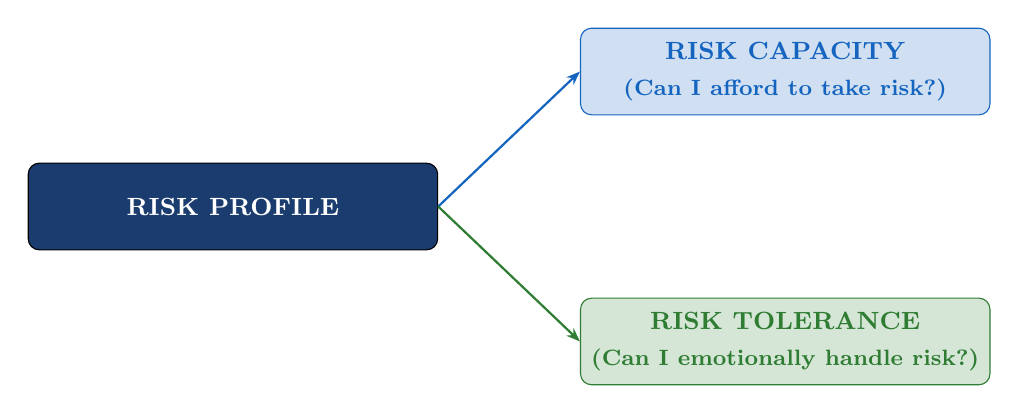
\begin{tikzpicture}[
  box/.style={draw, rounded corners=4pt, minimum width=5.2cm,
               minimum height=1.1cm, align=center, font=\small\bfseries},
  arr/.style={-{Stealth[length=5pt]}, thick}
]
  \node[box, fill=PrimaryBlue, text=white] (rp)
    {RISK PROFILE};
  \node[box, fill=CapacityColor!20, draw=CapacityColor,
        text=CapacityColor, above right=0.6cm and 1.8cm of rp] (rc)
    {RISK CAPACITY\\[2pt]\footnotesize(Can I afford to take risk?)};
  \node[box, fill=ToleranceColor!20, draw=ToleranceColor,
        text=ToleranceColor, below right=0.6cm and 1.8cm of rp] (rt)
    {RISK TOLERANCE\\[2pt]\footnotesize(Can I emotionally handle risk?)};
  \draw[arr, CapacityColor] (rp.east) -- (rc.west);
  \draw[arr, ToleranceColor] (rp.east) -- (rt.west);
\end{tikzpicture}
\end{center}

\vspace{2mm}

% ─────────────────────────────────────────────────────────────
\section{Pillar 1 --- Risk Capacity (The Financial Side)}
% ─────────────────────────────────────────────────────────────

\begin{definitionbox}{Risk Capacity}
\textbf{Risk Capacity} is the \textit{objective}, financially-grounded measure of how much risk you \textbf{can afford} to take, based on your real-world financial situation --- regardless of how you \textit{feel} about risk.
\end{definitionbox}

Think of it this way: a 22-year-old with no dependants, a stable job, and minimal expenses can afford to lose a portion of their investment without derailing their life. A 65-year-old retiree with limited savings simply cannot.

\subsection{The Four Drivers of Risk Capacity}

\begin{center}
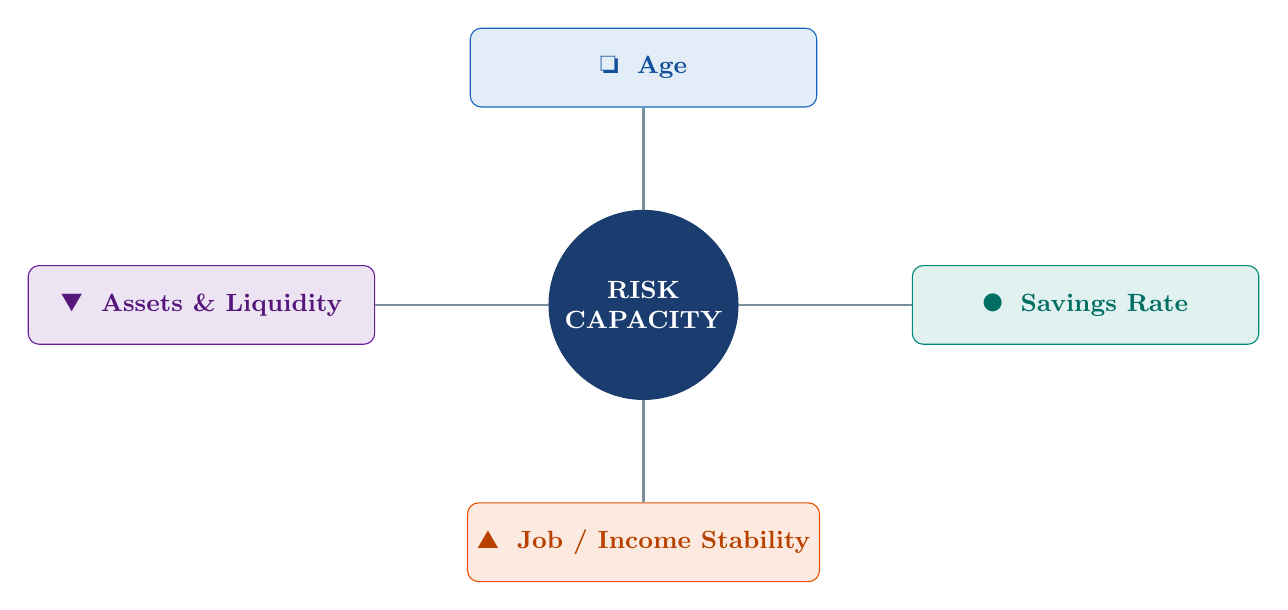
\begin{tikzpicture}[
  center/.style={circle, draw=PrimaryBlue, fill=PrimaryBlue,
                 text=white, font=\bfseries\small,
                 minimum width=2.4cm, align=center},
  leaf/.style={rectangle, rounded corners=4pt, draw=#1, fill=#1!12,
               text=#1!80!black, font=\small\bfseries,
               minimum width=4.4cm, minimum height=1.0cm, align=center},
  line/.style={thick, draw=MidGray}
]
  \node[center] (c) {RISK\\CAPACITY};

  \node[leaf=CapacityColor, above=1.3cm of c] (age)
    {\faCalendar\; Age};
  \node[leaf=AccentTeal, right=2.2cm of c] (sav)
    {\faPiggyBank\; Savings Rate};
  \node[leaf=AccentOrange, below=1.3cm of c] (job)
    {\faBriefcase\; Job / Income Stability};
  \node[leaf=AccentPurple, left=2.2cm of c] (ast)
    {\faChartLine\; Assets \& Liquidity};

  \draw[line] (c) -- (age);
  \draw[line] (c) -- (sav);
  \draw[line] (c) -- (job);
  \draw[line] (c) -- (ast);
\end{tikzpicture}
\end{center}

\vspace{3mm}

% --- Factor 1: Age ---
\begin{tcolorbox}[base, colback=CapacityColor!8, colframe=CapacityColor,
  title={\faCalendar\;\textbf{Factor 1: Age}},
  fonttitle=\bfseries\color{white}, colbacktitle=CapacityColor]

\textbf{Rule:} Higher the age $\longrightarrow$ Lower the risk capacity.

\medskip
As you get older, you have fewer earning years ahead and a more limited corpus. You rely more on your existing assets and cannot easily rebuild wealth if a risky investment fails.

\medskip
\begin{itemize}
  \item \textbf{Age 20--25:} ``Nothing to lose'' phase. Parents handle emergencies, education, and marriage costs. Whatever you earn and invest is truly surplus --- your risk capacity is at its peak.
  \item \textbf{Age 35--45:} Dependants, home loan, children's education. Risk capacity is moderate and context-dependent.
  \item \textbf{Age 60+:} Retirement phase. No regular salary income. Drawing down from a fixed corpus. Risk capacity is typically low --- even a well-intentioned equity bet can wipe out years of savings.
\end{itemize}

\medskip
\textit{A 70-year-old with limited savings should almost never be advised to go 100\% into equity --- regardless of how optimistic they feel.}
\end{tcolorbox}

\vspace{3mm}

% --- Factor 2: Savings Rate ---
\begin{tcolorbox}[base, colback=AccentTeal!8, colframe=AccentTeal,
  title={\faPiggyBank\;\textbf{Factor 2: Savings Rate}},
  fonttitle=\bfseries\color{white}, colbacktitle=AccentTeal]

\textbf{Rule:} Higher the savings rate $\longrightarrow$ Higher the risk capacity.

\medskip
If you are only saving 10--15\% of your income, every rupee saved is critical for meeting your goals (retirement, children's education, home). There is no room for big losses.

\medskip
If you save 50--60\% of your income and all major goals are already on track, the additional surplus can bear much higher risk --- because even if you lose it, your primary goals are unaffected.

\medskip
\textbf{Example:} Imagine someone saving \rupee{}30,000/month after expenses. If \rupee{}20,000 goes to long-term goals (SIPs, PPF, etc.) and \rupee{}10,000 is genuinely surplus, that extra \rupee{}10,000 can sustain much higher risk. But if someone barely saves \rupee{}5,000/month and invests it all in small-cap funds, even a 30\% drawdown could hurt them badly.
\end{tcolorbox}

\vspace{3mm}

% --- Factor 3: Job Stability ---
\begin{tcolorbox}[base, colback=AccentOrange!8, colframe=AccentOrange,
  title={\faBriefcase\;\textbf{Factor 3: Job / Income Stability}},
  fonttitle=\bfseries\color{white}, colbacktitle=AccentOrange]

\textbf{Rule:} More stable the income $\longrightarrow$ Higher the risk capacity.

\medskip
\begin{itemize}
  \item \textbf{Government employees / large IT companies:} Strong HR policies, virtually guaranteed paycheques. Risk capacity is higher because income disruption is unlikely.
  \item \textbf{Entrepreneurs / self-employed:} Income is irregular and unpredictable. Even if net worth is high, personal risk \textit{capacity} may be lower because next month's income is uncertain. They might not know whether they can sustain their SIP if a bad quarter hits.
  \item \textbf{Contract workers / gig economy:} Similar to entrepreneurs --- unpredictability reduces capacity.
\end{itemize}

\medskip
\textit{Note: This is about personal financial capacity, not the risk-taking personality of the entrepreneur. The bravest entrepreneur in business may still have low personal financial risk capacity.}
\end{tcolorbox}

\vspace{3mm}

% --- Factor 4: Assets & Liquidity ---
\begin{tcolorbox}[base, colback=AccentPurple!8, colframe=AccentPurple,
  title={\faChartLine\;\textbf{Factor 4: Assets \& Liquidity}},
  fonttitle=\bfseries\color{white}, colbacktitle=AccentPurple]

\textbf{Rule:} Higher the assets relative to your goals $\longrightarrow$ Higher the risk capacity.

\medskip
If someone has accumulated significant wealth (say, several crores of rupees in assets), and all major goals --- retirement corpus, children's education, home --- are already funded, then \textit{every additional rupee they invest is pure wealth creation}. That portion can afford to take aggressive risk.

\medskip
Conversely, if someone has liabilities (home loan, car loan, credit card debt) exceeding their assets, they have very low capacity to absorb any investment losses.

\medskip
\textbf{Quick check:} Net Worth = Total Investment Assets $-$ Total Liabilities. If this number barely covers a few months of expenses, risk capacity is very low.
\end{tcolorbox}

\vspace{3mm}

% ─────────────────────────────────────────────────────────────
\section{Pillar 2 --- Risk Tolerance (The Psychological Side)}
% ─────────────────────────────────────────────────────────────

\begin{definitionbox}{Risk Tolerance}
\textbf{Risk Tolerance} is the \textit{subjective}, psychological measure of how much volatility and uncertainty you can \textbf{emotionally handle} in your investments --- regardless of what your finances say.
\end{definitionbox}

This is the harder part to measure honestly. Markets tend to reveal your true risk tolerance very quickly --- especially during a crash.

\begin{examplebox}{The Sleep Test}
You invest \rupee{}1,00,000. The very next day, the market falls and your portfolio shows \rupee{}88,000. Ask yourself honestly:
\begin{itemize}
  \item Can you sleep soundly that night without worrying?
  \item Do you check your portfolio the next morning with curiosity (not panic)?
  \item Do you think, \textit{``Great, it's on sale --- let me invest more''?}
\end{itemize}
If yes to all three, your risk tolerance is \textbf{high}.

\medskip
But if you are:
\begin{itemize}
  \item Losing sleep thinking about the \rupee{}12,000 loss,
  \item Calling your friends or your advisor in a panic,
  \item Tempted to sell everything before it falls further,
\end{itemize}
\ldots then your risk tolerance is \textbf{low to moderate} --- regardless of how much money you actually have.
\end{examplebox}

\vspace{2mm}

\subsection{The Three Tolerance Profiles}

\begin{center}
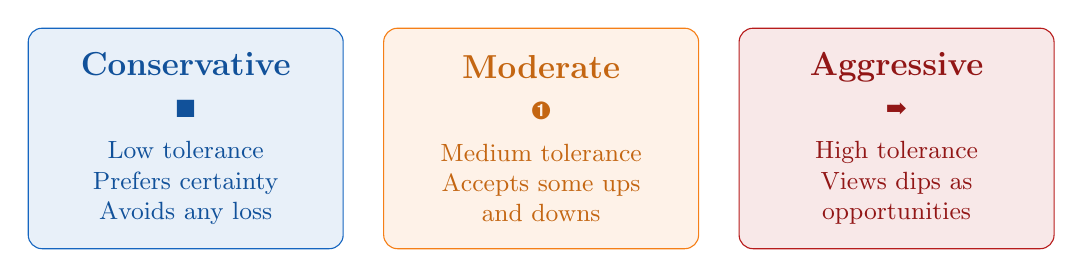
\begin{tikzpicture}[
  node distance=0.2cm,
  box/.style={rectangle, rounded corners=5pt, draw=#1,
    fill=#1!10, text=#1!80!black,
    minimum width=4.0cm, minimum height=2.8cm,
    align=center, font=\small}
]
  \node[box=Conservative] (con) {%
    \textbf{\large Conservative}\\[4pt]
    \faShield\\[4pt]
    Low tolerance\\
    Prefers certainty\\
    Avoids any loss
  };
  \node[box=Moderate, right=0.5cm of con] (mod) {%
    \textbf{\large Moderate}\\[4pt]
    \faBalanceScale\\[4pt]
    Medium tolerance\\
    Accepts some ups\\
    and downs
  };
  \node[box=Aggressive, right=0.5cm of mod] (agg) {%
    \textbf{\large Aggressive}\\[4pt]
    \faRocket\\[4pt]
    High tolerance\\
    Views dips as\\
    opportunities
  };
\end{tikzpicture}
\end{center}

\vspace{3mm}

% Conservative
\begin{tcolorbox}[base, colback=Conservative!8, colframe=Conservative,
  title={\faShield\;\textbf{Conservative (Low Tolerance)}},
  fonttitle=\bfseries\color{white}, colbacktitle=Conservative]

\textbf{Who they are:} Investors who are deeply uncomfortable with any loss, even temporary. They prefer knowing exactly what they will get back.

\medskip
\textbf{Behaviour:} Even if they \textit{can} afford to take risk (high capacity), they choose not to. They feel better with FDs, government bonds, liquid funds, or debt mutual funds.

\medskip
\textbf{Example:} \textit{Ashish, 50 years old, 10 years from retirement. He has some savings but doesn't want to see his retirement corpus fluctuate. He puts his money in fixed deposits and short-duration debt funds.} He values certainty over higher returns.

\medskip
\textbf{Not wrong!} Being conservative is a valid choice --- as long as you account for inflation eating into your returns over time.
\end{tcolorbox}

\vspace{3mm}

% Moderate
\begin{tcolorbox}[base, colback=Moderate!8, colframe=Moderate,
  title={\faBalanceScale\;\textbf{Moderate (Medium Tolerance)}},
  fonttitle=\bfseries\color{white}, colbacktitle=Moderate]

\textbf{Who they are:} The largest group of investors. They can accept \textit{some} market ups and downs but start to feel uneasy during big corrections.

\medskip
\textbf{Behaviour (a real-world marker):} During a market fall, they do \textbf{not sell} --- but they do start checking their portfolio daily, asking questions, and discussing the losses with friends. They hold on, but they are not comfortable.

\medskip
\textbf{Example:} \textit{Gaurav, 35 years old, investing for his daughter's higher education in 10 years. He wants growth but cannot risk losing the core corpus. He invests in balanced/hybrid mutual funds and large-cap stocks.}

\medskip
\textbf{Reality check:} Most people who think they are aggressive investors are actually moderate. The true test comes when the market falls 20--30\%.
\end{tcolorbox}

\vspace{3mm}

% Aggressive
\begin{tcolorbox}[base, colback=Aggressive!8, colframe=Aggressive,
  title={\faRocket\;\textbf{Aggressive (High Tolerance)}},
  fonttitle=\bfseries\color{white}, colbacktitle=Aggressive]

\textbf{Who they are:} Investors who are genuinely \textit{excited} when markets fall. They see a 20\% drop as a discount sale, not a disaster.

\medskip
\textbf{Behaviour:} They have a long time horizon (8--10+ years), maintain a cash reserve specifically to invest during corrections, and their portfolio allocation does not change during a crash.

\medskip
\textbf{Example:} \textit{Sanjay, 25 years old, goal of wealth creation over 15 years. He has a stable job, no major dependants, and a diversified emergency fund. He invests in small-cap and thematic mutual funds, knowing they can fall 40--50\% --- and he is mentally prepared for that.}

\medskip
\textbf{Warning:} Do not confuse aggressive \textit{aspiration} with aggressive \textit{tolerance}. Wanting high returns is not the same as being able to handle a 40\% drawdown without panic.
\end{tcolorbox}

\vspace{3mm}

% ─────────────────────────────────────────────────────────────
\section{The Critical Intersection: Capacity vs.\ Tolerance}
% ─────────────────────────────────────────────────────────────

This is the most important conceptual point of this chapter. Your risk \textit{capacity} and risk \textit{tolerance} are \textbf{two separate things}, and they can (and often do) disagree.

\begin{center}
\begin{tabular}{B{3.8cm} L{4.5cm} L{5.2cm}}
\toprule
Scenario & What it means & What to do\\
\midrule
\rowcolor{LightGreen}
High Capacity + High Tolerance
& Both financial ability and emotional comfort support aggressive investing.
& You can allocate meaningfully to equity, small-cap, etc.\\[6pt]

\rowcolor{LightBlue}
High Capacity + Low Tolerance
& You \textit{can} afford risk but \textit{don't want to} take it.
& Respect your comfort. Start with moderate options. Gradually build market knowledge to raise tolerance.\\[6pt]

\rowcolor{LightOrange}
Low Capacity + High Tolerance
& You \textit{want} to take risk but \textit{cannot afford} to.
& \textbf{Be careful.} This is the most dangerous combination. High ambition + low financial cushion = potential disaster.\\[6pt]

\rowcolor{LightRed}
Low Capacity + Low Tolerance
& Neither financial nor emotional support for risk.
& Stick to conservative options. Focus first on building savings rate and emergency fund.\\
\bottomrule
\end{tabular}
\end{center}

\vspace{3mm}

\begin{warningbox}
The \textbf{most dangerous combination} is \textit{Low Capacity + High Tolerance}. Many new investors in bull markets fall into this trap --- they feel brave because markets have only gone up for the past 2 years, so they invest aggressively beyond their financial means. When the market corrects, they cannot afford to hold on and are forced to sell at losses.
\end{warningbox}

% ─────────────────────────────────────────────────────────────
\section{Measuring Your Risk Profile: The Structured Test}
% ─────────────────────────────────────────────────────────────

Below is a structured Risk Analysis Test with two sections. Answer honestly --- the goal is insight, not a high score.

\subsection{Part A --- Financial Risk Capacity (Max 18 points)}

\begin{tcolorbox}[base, colback=CapacityColor!7, colframe=CapacityColor, breakable]
\textbf{\color{CapacityColor}Q1. What is your Net Worth relative to monthly expenses?}\\
\textit{(Net Worth = Total Investment Assets $-$ Total Liabilities)}

\medskip
\begin{tabular}{ll}
\textbf{A.} Only liabilities (net worth is negative) & 1 point\\
\textbf{B.} Up to 12$\times$ monthly expenses & 2 points\\
\textbf{C.} 13$\times$ to 36$\times$ monthly expenses & 3 points\\
\textbf{D.} 37$\times$ to 48$\times$ monthly expenses & 4 points\\
\textbf{E.} 49$\times$ to 60$\times$ monthly expenses & 5 points\\
\end{tabular}

\bigskip
\textbf{\color{CapacityColor}Q2. What is your monthly Income Saving Rate?}

\medskip
\begin{tabular}{ll}
\textbf{A.} Up to 5\% & 1 point\\
\textbf{B.} 6\%--15\% & 2 points\\
\textbf{C.} 16\%--25\% & 3 points\\
\textbf{D.} 26\%--50\% & 4 points\\
\textbf{E.} 51\%--75\% & 5 points\\
\end{tabular}

\bigskip
\textbf{\color{CapacityColor}Q3. How many people are financially dependent on your income?}

\medskip
\begin{tabular}{ll}
\textbf{A.} No one & 5 points\\
\textbf{B.} One person & 4 points\\
\textbf{C.} Two people & 3 points\\
\textbf{D.} Three people & 2 points\\
\textbf{E.} Four or more & 1 point\\
\end{tabular}

\bigskip
\textbf{\color{CapacityColor}Q4. How stable/consistent is your job or income for the next year?}

\medskip
\begin{tabular}{ll}
\textbf{A.} High (government job, large stable company) & 3 points\\
\textbf{B.} Moderate (somewhat unsatisfied / company instability) & 2 points\\
\textbf{C.} Low (fear of job loss / highly variable income) & 1 point\\
\end{tabular}
\end{tcolorbox}

\vspace{2mm}

\begin{tcolorbox}[base, colback=CapacityColor!7, colframe=CapacityColor]
\centering
\textbf{\color{CapacityColor}Financial Risk Capacity Scoring Table}

\medskip
\begin{tabular}{cc}
\toprule
\textbf{Total Score} & \textbf{Risk Capacity Level}\\
\midrule
4--7 & Very Low\\
8--11 & Low\\
12--14 & Moderate\\
15--16 & High\\
17--18 & Very High\\
\bottomrule
\end{tabular}

\medskip
\textit{My Financial Risk Capacity Score: }\underline{\hspace{2cm}}
\quad
\textit{Level: }\underline{\hspace{3cm}}
\end{tcolorbox}

\vspace{4mm}

\subsection{Part B --- Psychological Risk Tolerance (Max 15 points)}

\begin{tcolorbox}[base, colback=ToleranceColor!7, colframe=ToleranceColor, breakable]
\textbf{\color{ToleranceColor}Q1. How would you rate your current level of market/investing knowledge?}

\medskip
\begin{tabular}{ll}
\textbf{A.} No knowledge & 1 point\\
\textbf{B.} Beginner (have read a few articles) & 2 points\\
\textbf{C.} Intermediate (understand market cycles, fund categories) & 3 points\\
\textbf{D.} Expert (understand valuations, portfolio theory) & 4 points\\
\textbf{E.} Professional (work in finance / deep expertise) & 5 points\\
\end{tabular}

\bigskip
\textit{Why does knowledge matter?} Because the more you understand why markets fall, the less likely you are to panic when they do. Knowledge directly raises emotional tolerance.

\bigskip
\textbf{\color{ToleranceColor}Q2. What is the maximum monthly portfolio decline you could tolerate without losing sleep?}

\medskip
\begin{tabular}{ll}
\textbf{A.} 0--5\% & 1 point\\
\textbf{B.} 6--10\% & 2 points\\
\textbf{C.} 11--20\% & 3 points\\
\textbf{D.} 21--30\% & 4 points\\
\textbf{E.} More than 30\% & 5 points\\
\end{tabular}

\bigskip
\textbf{\color{ToleranceColor}Q3. If your investment shows a negative return, how long can you hold without acting on that discomfort?}

\medskip
\begin{tabular}{ll}
\textbf{A.} Less than 3 months & 1 point\\
\textbf{B.} 4 months to 1 year & 2 points\\
\textbf{C.} 1--2 years & 3 points\\
\textbf{D.} 2--3 years & 4 points\\
\textbf{E.} 3--5 years & 5 points\\
\end{tabular}
\end{tcolorbox}

\vspace{2mm}

\begin{tcolorbox}[base, colback=ToleranceColor!7, colframe=ToleranceColor]
\centering
\textbf{\color{ToleranceColor}Psychological Risk Tolerance Scoring Table}

\medskip
\begin{tabular}{cc}
\toprule
\textbf{Total Score} & \textbf{Risk Tolerance Level}\\
\midrule
3--5 & Very Low\\
6--8 & Low\\
9--11 & Moderate\\
12--13 & High\\
14--15 & Very High\\
\bottomrule
\end{tabular}

\medskip
\textit{My Psychological Risk Tolerance Score: }\underline{\hspace{2cm}}
\quad
\textit{Level: }\underline{\hspace{3cm}}
\end{tcolorbox}

\vspace{2mm}

\begin{keybox}
After completing both sections, compare your two levels. Your overall risk profile is determined by \textbf{the lower of the two scores}. For example, if your capacity is \textit{High} but your tolerance is \textit{Low}, your effective investment risk profile is \textit{Low}. Never let capacity override tolerance --- you must be able to \textit{sleep at night} with your investments.
\end{keybox}

% ─────────────────────────────────────────────────────────────
\section{Online Risk Profiling Tools}
% ─────────────────────────────────────────────────────────────

If you prefer a guided online experience, several free tools are available:

\begin{itemize}
  \item \textbf{InvestYadnya (investyadnya.in):} Offers a detailed risk profiling questionnaire as part of their free financial planning tool. The tool also generates a complete financial plan when you input your assets and goals, giving you both a capacity-based and questionnaire-based risk profile to compare.

  \item \textbf{General online risk calculators:} Many AMC websites and personal finance portals offer free risk profiling tools. Look for one that does \textit{not} ask for personal contact details upfront (to avoid unsolicited sales calls). A good tool asks 5--8 questions covering your finances, timeline, and emotional reactions to hypothetical market scenarios.
\end{itemize}

\textbf{Sample questions from a good profiling tool:}
\begin{enumerate}
  \item What is your \textit{first instinct} when making an investment? (Caution vs.\ opportunity)
  \item What does the word \textit{risk} mean to you? (Danger vs.\ opportunity vs.\ thrill)
  \item Would you rather start a business or take a salaried job?
  \item What \% of your portfolio would you expose to risk for higher returns?
  \item How would you \textit{feel} if your recent investments underperformed?
  \item Would you re-invest in a fund that caused you losses in the past?
\end{enumerate}

% ─────────────────────────────────────────────────────────────
\section{Risk Levels in Mutual Fund Schemes}
% ─────────────────────────────────────────────────────────────

Once you know your risk profile, the next question is: \textit{which category of mutual fund corresponds to which level of risk?}

\subsection{Six Fundamental Rules of Fund Risk}

\begin{enumerate}[leftmargin=*, label=\textbf{\arabic*.}]
  \item \textbf{Equity is more risky than Debt.}\\
  Equity funds invest in shares of companies. Their value rises and falls with the stock market. Debt funds invest in bonds and government securities --- much more stable, but lower returns.

  \item \textbf{Concentrated funds are riskier than Diversified funds.}\\
  A fund investing in 10--15 stocks in one sector is far more exposed to a single adverse event than a fund spread across 50--100 stocks in multiple sectors.

  \item \textbf{As Debt Duration increases, Interest Rate risk increases.}\\
  A long-duration debt fund holds bonds maturing 10--15 years from now. If interest rates rise, those bond prices fall sharply. A liquid fund or overnight fund holds instruments maturing in days --- virtually no interest rate risk.

  \item \textbf{Credit Risk depends on the credibility of the issuer.}\\
  A gilt fund holds only government bonds --- near-zero credit risk (the government won't default). A credit risk fund holds bonds from lower-rated companies with higher yields but meaningful default risk.

  \item \textbf{Small-cap funds are riskier than Large-cap funds.}\\
  Small-cap companies are less established, less liquid, and more volatile. Large-cap companies have proven business models and are more resilient during market crashes.

  \item \textbf{Aggressive funds are riskier than Conservative funds.}\\
  Within hybrid funds, aggressive hybrid funds tilt heavily towards equity ($\approx$65--80\%) while conservative hybrid funds tilt towards debt ($\approx$75--90\%).
\end{enumerate}

\vspace{3mm}

\subsection{Risk\textendash{}Return Hierarchy by Fund Category}

\begin{center}
\begingroup
\small
\renewcommand{\arraystretch}{1.12}
\setlength{\tabcolsep}{5pt}
\begin{tabularx}{\linewidth}{B{3.6cm} Y}
\toprule
\rowcolor{PrimaryBlue}
\textcolor{white}{\textbf{Category}} &
\textcolor{white}{\textbf{Risk Hierarchy (Low \texorpdfstring{$\longrightarrow$}{to} High)}}\\
\midrule
\rowcolor{LightGreen}
All Mutual Funds
& \textcolor{ToleranceColor}{\textbf{Liquid Funds}} $\to$ Debt Funds $\to$ Hybrid Funds $\to$ \textcolor{Aggressive}{\textbf{Equity Funds}}\\[5pt]

\rowcolor{LightBlue}
Debt Funds\\[-1pt]{\normalfont\small Duration / Interest Rate Risk}
& \textcolor{ToleranceColor}{\textbf{Overnight Funds}} $\to$ Liquid Funds $\to$ Ultra Short Duration $\to$ Low Duration $\to$ Short Duration $\to$ Medium Duration $\to$ Medium-to-Long Duration $\to$ \textcolor{Aggressive}{\textbf{Long Duration}}\\[5pt]

\rowcolor{LightPurple}
Debt Funds\\[-1pt]{\normalfont\small Issuer / Credit Risk}
& \textcolor{ToleranceColor}{\textbf{Gilt Funds}} $\to$ Banking \& PSU Funds $\to$ Corporate Bond Funds $\to$ \textcolor{Aggressive}{\textbf{Credit Risk Funds}}\\[5pt]

\rowcolor{LightOrange}
Equity Mutual Funds
& \textcolor{ToleranceColor}{\textbf{Large-Cap Funds}} $\to$ Large \& Mid-Cap Funds $\to$ Multi-Cap Funds $\to$ Mid-Cap Funds $\to$ \textcolor{Aggressive}{\textbf{Small-Cap Funds}}\\[5pt]

\rowcolor{LightRed}
Diversification Level
& \textcolor{ToleranceColor}{\textbf{Diversified Funds}} $\to$ Focused Funds $\to$ Thematic Funds $\to$ \textcolor{Aggressive}{\textbf{Sector Funds}}\\[5pt]

\rowcolor{SoftGray}
Hybrid Funds
& \textcolor{ToleranceColor}{\textbf{Arbitrage Funds}} $\to$ Equity Savings Funds $\to$ Conservative Hybrid $\to$ Dynamic Asset Allocation $\to$ Multi Asset Allocation $\to$ Balanced Hybrid $\to$ \textcolor{Aggressive}{\textbf{Aggressive Hybrid}}\\
\bottomrule
\end{tabularx}
\endgroup
\end{center}

\vspace{3mm}

\subsection{The Riskometer: India's Mandatory Risk Label}

Every mutual fund in India is required by SEBI to display a \textbf{Riskometer} on its product label --- a speedometer-shaped graphic that classifies the fund's risk level into one of six categories:

\begin{center}
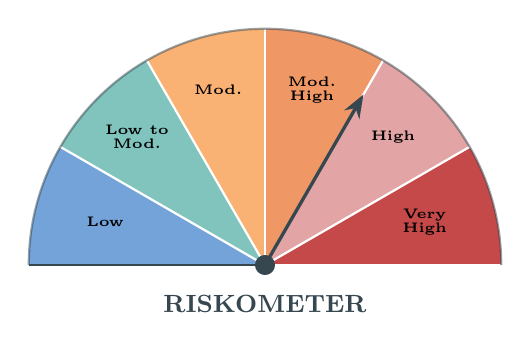
\begin{tikzpicture}[scale=1.0]
  % Draw the speedometer arc
  \def\R{3.0}
  % Segments from left to right: Low, Low-Mod, Mod, Mod-High, High, V.High
  \foreach \start/\end/\col/\lbl in {%
    180/150/Conservative!60!white/Low,
    150/120/AccentTeal!50!white/Low to Moderate,
    120/90/Moderate!60!white/Moderate,
    90/60/AccentOrange!60!white/Moderately High,
    60/30/Aggressive!40!white/High,
    30/0/Aggressive!80!white/Very High}
  {%
    \fill[\col] (0,0) -- (\start:\R) arc(\start:\end:\R) -- cycle;
    \draw[white, thick] (0,0) -- (\start:\R);
  }
  \draw[white, thick] (0,0) -- (0:\R);
  \draw[DarkGray, thick] (0,0) -- (180:\R);
  % Labels
  \node[font=\tiny\bfseries, align=center] at (165:2.1) {Low};
  \node[font=\tiny\bfseries, align=center] at (135:2.3) {Low to\\[-1pt]Mod.};
  \node[font=\tiny\bfseries, align=center] at (105:2.3) {Mod.};
  \node[font=\tiny\bfseries, align=center] at (75:2.3) {Mod.\\[-1pt]High};
  \node[font=\tiny\bfseries, align=center] at (45:2.3) {High};
  \node[font=\tiny\bfseries, align=center] at (15:2.1) {Very\\[-1pt]High};
  % Needle
  \draw[-{Stealth}, very thick, DarkGray] (0,0) -- (60:2.5);
  % Base
  \filldraw[DarkGray] (0,0) circle (0.12);
  % Label
  \node[font=\bfseries\small, DarkGray] at (0,-0.5) {RISKOMETER};
  % Bottom arc
  \draw[DarkGray, thick, semitransparent]
    (180:\R) arc (180:0:\R);
\end{tikzpicture}
\end{center}

\begin{itemize}
  \item \textbf{Purpose:} Prevents mis-selling by ensuring every investor knows the risk level of a fund before investing.
  \item \textbf{How to use it:} Match the Riskometer level of a fund to your own risk profile. A Very High riskometer fund should only be bought by investors with an Aggressive profile.
\end{itemize}

% ─────────────────────────────────────────────────────────────
\section{Matching Your Risk Profile to the Right Fund Type}
% ─────────────────────────────────────────────────────────────

\begin{center}
\begin{tabular}{B{2.8cm} L{3.2cm} L{3.2cm} L{4.2cm}}
\toprule
\textbf{Risk Profile} & \textbf{Suitable Fund Categories} & \textbf{Example Investor} & \textbf{Typical Instruments}\\
\midrule
\rowcolor{Conservative!10}
Conservative
& Debt Funds, Liquid Funds, Overnight Funds
& Ashish, 50 yrs,\newline retirement in 10 yrs
& Fixed deposits, government bonds, short-duration debt\\[6pt]

\rowcolor{Moderate!10}
Moderate
& Large-Cap Equity, Balanced/Hybrid Funds
& Gaurav, 35 yrs,\newline daughter's education
& Large-cap stocks, balanced hybrid, multi-asset\\[6pt]

\rowcolor{Aggressive!10}
Aggressive
& Mid-Cap, Small-Cap, Thematic, Sector Funds
& Sanjay, 25 yrs,\newline long-term wealth creation
& Small-cap stocks, thematic funds, high-risk MFs\\
\bottomrule
\end{tabular}
\end{center}

% ─────────────────────────────────────────────────────────────
\section{Risk Profile Is Not Fixed for Life}
% ─────────────────────────────────────────────────────────────

\begin{conceptbox}{Risk Profiles Change Over Time}
Your risk profile is \textbf{not a one-time label}. It should be revisited periodically (ideally once a year) and also whenever a major life event occurs.
\end{conceptbox}

\textbf{Events that commonly shift your risk profile:}
\begin{itemize}
  \item \textbf{Getting married} --- new shared financial goals, potentially reduced risk capacity.
  \item \textbf{Having a child} --- new long-term expense obligations, education planning.
  \item \textbf{Job change or loss} --- income stability drops, capacity drops.
  \item \textbf{Major business loss} --- net worth and savings rate both affected.
  \item \textbf{Inheritance or large windfall} --- capacity may increase significantly.
  \item \textbf{Approaching retirement} --- both capacity and ideal tolerance should decrease.
  \item \textbf{Increased market knowledge} --- tolerance can increase as understanding deepens.
\end{itemize}

\vspace{2mm}

\begin{keybox}
The single most powerful way to raise your \textit{psychological} risk tolerance without changing your financial situation is to \textbf{increase your market knowledge}. The more you understand why markets fall and recover, the less frightened you will be during downturns. This is exactly why financial literacy matters.
\end{keybox}

% ─────────────────────────────────────────────────────────────
\section{The Role of an Unbiased External Opinion}
% ─────────────────────────────────────────────────────────────

Research consistently shows that people are \textbf{poor judges of their own risk tolerance} --- particularly before they have experienced a real market crash. Most new investors overestimate their tolerance during bull markets.

This is why a good, unbiased financial advisor is valuable:
\begin{itemize}
  \item They can observe your actual behaviour (not just your stated preference) and calibrate accordingly.
  \item They can separate \textit{feeling brave} from \textit{genuinely being able to handle a 40\% drawdown}.
  \item They can update your profile after life events that you might not think to report.
\end{itemize}

\textbf{If you don't have an advisor:} Use a structured questionnaire (like the one above), be rigorously honest, and revisit it every year.

% ─────────────────────────────────────────────────────────────
\section*{Chapter Summary \& Cheat Sheet}
% ─────────────────────────────────────────────────────────────
\addcontentsline{toc}{section}{Chapter Summary \& Cheat Sheet}

\begin{cheatsheet}

\textbf{\color{PrimaryBlue}\large Step 1: Understand the Two Pillars}

\medskip
\begin{tabular}{p{0.45\linewidth} p{0.45\linewidth}}
\textbf{Risk Capacity} (Financial) & \textbf{Risk Tolerance} (Psychological)\\
Can you \textit{afford} to take risk? & Can you \textit{emotionally handle} risk?\\
Based on age, savings, job stability, assets & Based on market knowledge, reaction to losses, holding ability\\
Objective --- facts-based & Subjective --- feelings-based\\
\end{tabular}

\bigskip
\textbf{\color{PrimaryBlue}\large Step 2: Score Yourself}

\medskip
\begin{tabular}{lll}
\textbf{Section} & \textbf{Max Score} & \textbf{Your Score}\\
Financial Capacity (4 questions) & 18 & \underline{\hspace{1.5cm}}\\
Psychological Tolerance (3 questions) & 15 & \underline{\hspace{1.5cm}}\\
\end{tabular}

\bigskip
\textbf{\color{PrimaryBlue}\large Step 3: Identify Your Profile}

\medskip
\begin{tabular}{p{0.3\linewidth} p{0.3\linewidth} p{0.3\linewidth}}
\textbf{Conservative} & \textbf{Moderate} & \textbf{Aggressive}\\
Debt / Liquid Funds & Hybrid / Large-Cap & Small-Cap / Thematic\\
Safety first & Balanced growth & Maximum growth\\
\end{tabular}

\bigskip
\textbf{\color{PrimaryBlue}\large Six Rules to Remember}

\begin{enumerate}[label=\textbf{\arabic*.}, leftmargin=*]
  \item Equity $>$ Debt in risk.
  \item Concentrated funds $>$ Diversified funds in risk.
  \item Longer debt duration = Higher interest rate risk.
  \item Lower issuer credit rating = Higher credit risk.
  \item Small-cap $>$ Large-cap in risk.
  \item Aggressive hybrid $>$ Conservative hybrid in risk.
\end{enumerate}

\bigskip
\textbf{\color{PrimaryBlue}\large Remember:}
\begin{itemize}
  \item Your effective profile = \textit{lower} of capacity and tolerance.
  \item Revisit your profile \textbf{once a year} or after any major life event.
  \item Knowledge is the best way to raise your tolerance.
  \item The Riskometer on every fund label helps you match the fund to your profile.
\end{itemize}

\end{cheatsheet}

\end{document}
